\chapter{ОЗНАКОМЛЕНИЕ С ПРОГРАММНЫМ ОБЕСПЕЧЕНИЕМ}
OWEN Logic --- среда программирования, предназначенная для создания алгоритмов работы коммутационных приборов, программируемых логических контроллеров, относящихся к классу программируемых реле, в частности, приборов серий ПР1хх, ПР200 и панели ИПП120 производства компании ОВЕН. Программируемые логические контроллеры (далее ПЛК) -- это свободно программируемое устройство. Алгоритм работы ПЛК формируется непосредственно пользователем, что делает прибор универсальным и дает возможность широко использовать его в различных областях.

OWEN Logic позволяет пользователю разработать программу автоматизации системы по собственному алгоритму и записать ее в энергонезависимую память прибора. Для составления программы используется графический язык FBD, который применяется в цифровых электрических схемах. Также присутствует возможность создания блоков-макросов на языке ST или FBD.

Для работы OWEN Logic требуется операционная система Windows XP/7/8/10 и программная платформа «.NET Framework» версии 4.0. или выше.

\begin{figure}[hb]
    \centering
    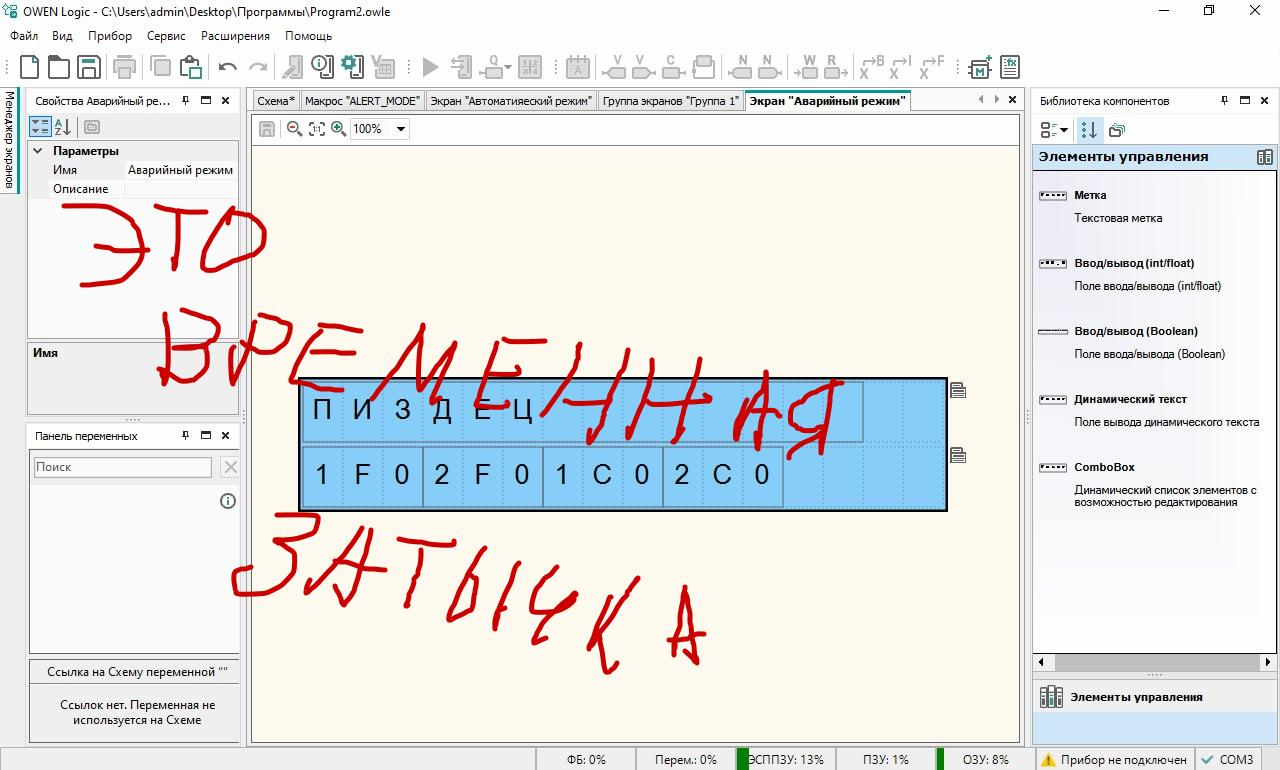
\includegraphics[scale=0.30]{fig/4.1.jpg}
    \caption{Интерфейс программы Owen Logic}
    \label{fig:owenlogic}
\end{figure}

\newpage
\section{Описание интерфейса}
Главное окно содержит:
\begin{itemize}
    \item Главное меню: Файл, Вид, Прибор, Сервис, Расширения, Помощь
    \item Панели инструментов
    \item Панели Библиотека компонентов, Свойства и Переменные (до открытия или создания проекта в них нет информации)
    \item Рабочую область проекта -- поле редактирования программы (до открытия или создания проекта пустое)
    \item Строку состояния в нижней части главного окна, показывающую информация о доступных ресурсах прибора и подключении к OWEN Logic
    \item Менеджер экранов
\end{itemize}

\section{Принцип выполнения программы}
Программа для прибора составляется с учетом количества имеющихся у него входов, выходов и наличия часов реального времени.

Работу прибора можно представить в виде последовательно выполняемых шагов (рабочий цикл):
\begin{enumerate}
    \item Логическое состояние входов автоматически записывается в ячейки памяти входов (количество ячеек равно числу входов -- I1\dots In).
    \item Программа считывает значения из ячеек памяти входов и выполняет над ними логические операции в соответствии с алгоритмом работы.
    \item После обработки всей программы результаты записываются на физические выходы прибора (для включения выходных элементов Q1\dots Q4).
    \item Переход к Шагу 1 (после выполнения всех предыдущих шагов обработки программы цикл работы прибора повторяется с первого шага).
\end{enumerate}
Время выполнения всех шагов зависит от сложности алгоритма программы.